\documentclass[a4paper]{article}
\usepackage{amsfonts}
\usepackage{amsmath}
\usepackage{amssymb}
\usepackage{graphicx}  
\usepackage{cancel}

\newcommand{\degree}{^{\circ}}
\newcommand{\cis}{\operatorname{cis}}
\newcommand{\Bgsin}{\operatorname{Bgsin}}
\newcommand{\Bgcos}{\operatorname{Bgcos}}
\newcommand{\Bgtan}{\operatorname{Bgtan}}
\newcommand{\limit}{\lim\limits}
\newcommand{\summation}{\displaystyle\sum}
\newcommand{\dom}{\operatorname{dom}}
\newcommand{\Int}{\displaystyle\int}

\begin{document}
  
\noindent \large Auteur: Rune Suy \\
\noindent \large Studierichting: Informatica\\
\noindent \large Oefeningenreeks 5G nr. 3.2\\

\medskip

\normalsize

$f(x) = \dfrac{1}{x}$ over $[1, +\infty]$\\

$V = \pi \Int_1^{+\infty} \dfrac{1}{x^2}dx = \pi \limit_{b\rightarrow+\infty} \left[\dfrac{-1}{x}\right]_1^b = \pi \limit_{b\rightarrow+\infty}\left( \dfrac{-1}{b} + 1 \right) = \pi $\\

\begin{figure}[h]
\centering
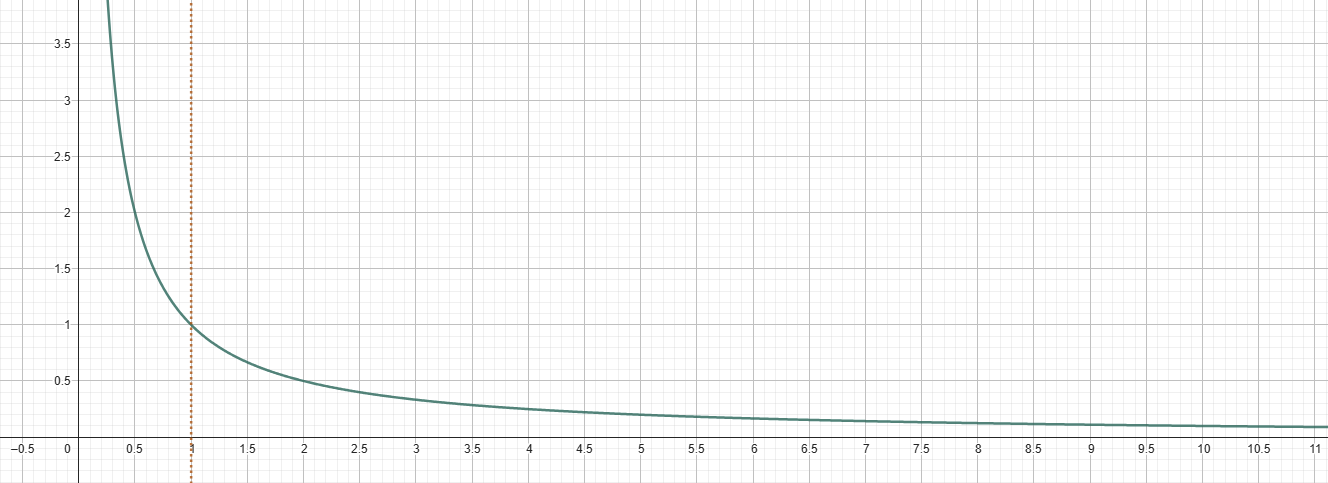
\includegraphics[width=\linewidth]{5G-3.2-rune.suy.INF.png}
\end{figure}

\begin{thebibliography}{999}
%\bibitem{a} Referentie
\end{thebibliography}
\end{document} 
